
\begin{figure}[htb]
\centering
\begin{tikzpicture}[scale = 10]
\tikzstyle{VertexStyle}=[shape = circle,	
								 minimum size = 1pt,
								 inner sep = 1.2pt,
                         draw]
\Vertex[x = 0.481999963521957, y = 0.880285702645779, L = \tiny {$y_1$}]{v0}
\Vertex[x = 0.451999992132187, y = 0.801428586244583, L = \tiny {$y_2$}]{v1}
\Vertex[x = 0.513999998569489, y = 0.801428586244583, L = \tiny {$y_3$}]{v2}
\Vertex[x = 0.482000023126602, y = 0.720285713672638, L = \tiny {$y_4$}]{v3}
\Edge[](v1)(v0)
\Edge[](v2)(v0)
\end{tikzpicture}
\caption{The antipaw.}
\label{fig:antipaw}
\end{figure}
